
%------------------------------------------------------------------------
\begin{frame}[fragile]
	\frametitle{Derivation in Damiani's \emph{Stingray}}
	Consider the aggregate realization A.
	\begin{equation*}
	\begin{adjustbox}{height=3.2cm}
		$A = \begin{tikzcd}
			& 0 \arrow[dddr] && 1 \arrow[dddr] & \\
			& 4 \arrow[ddr] && 5 \arrow[ddr] & \\
			& 8 \arrow[dr] && 9 \arrow[dr] & \\
    		* \arrow[ur] \arrow[uur] \arrow[uuur] \arrow[dr] \arrow[ddr] \arrow[dddr] && * \arrow[ur] \arrow[uur] \arrow[uuur] \arrow[dr] \arrow[ddr] \arrow[dddr] && * \\
    		& 11 \arrow[ur] && 10 \arrow[ur] & \\
    		& 7 \arrow[uur] && 6 \arrow[uur] & \\
    		& 3 \arrow[uuur] && 2 \arrow[uuur] &
    	\end{tikzcd}$
    \end{adjustbox}
	\end{equation*}
\end{frame}

%------------------------------------------------------------------------
\begin{frame}
	\frametitle{Derivation in Damiani's \emph{Stingray}}
	$A$ is invariant under the set of operations $\Omega = \{ \T_0, \T_4, \T_8, \T_3\I, \T_7\I, \T_{11}\I \}$. Thus if $\rho \in \Toc(A)$, then also $\Omega_i(\rho) \in \Toc(A)$. Also, $\R(\rho) \in \Toc(\R \circ \Omega_i(A))$. Let $S = \{ 0, 1, 5, 8, 9, 4, 10, 3, 7, 6, 2, 11 \}$, and consider $\mathcal{A} = [\mathcal{A}_1 | \cdots | \mathcal{A}_6]$.
	\begin{equation*}
    	\mathcal{A} = \left[
    	\begin{array}{cc|cc|cc|cc|cc|cc}
    		0 & 1 & 5 & 8 & 9 & 4 & 10 & 3 & 7 & 6 & 2 & 11 \\
    		4 & 5 & 9 & 0 & 1 & 8 & 2 & 7 & 11 & 10 & 6 & 3 \\
    		8 & 9 & 1 & 4 & 5 & 0 & 6 & 11 & 3 & 2 & 10 & 7 \\
    		11 & 10 & 6 & 3 & 2 & 7 & 1 & 8 & 4 & 5 & 9 & 0 \\
    		7 & 6 & 2 & 11 & 10 & 3 & 9 & 4 & 0 & 1 & 5 & 8 \\
    		3 & 2 & 10 & 7 & 6 & 11 & 5 & 0 & 8 & 9 & 1 & 4
    	\end{array}
    	\right]
	\end{equation*}
\end{frame}

%------------------------------------------------------------------------
\begin{frame}
	\frametitle{Derivation in Damiani's \emph{Stingray}}
	Every row of $\mathcal{A}$ is an $\Omega$-transform of $S$. Every $\mathcal{A}_i$ is an instance of either $A$ or $\R(A)$, thus $\Omega$-invariant. We can derive a transform of $S$ from every $\mathcal{A}_i$. Since $\T_7(S) \in \Toc(\mathcal{A}_1)$ and $\R\T_0\I(S) \in \Toc(\mathcal{A}_2)$, we get $X$.
	\begin{equation*}
	\begin{adjustbox}{width=\textwidth}
    	$X = \left[
    	\begin{array}{cccccccccccc|cccccccccccc}
    		&&&&& 11 && 10 &&&&&&& 6 &&&&& 3 &&&& \\
    		&&&& 4 && 5 &&&&&&&&&& 9 &&&&&&& 0 \\
    		&&& 3 &&&&& 2 &&&&& 10 &&&&&&&& 7 && \\
    		&& 0 &&&&&&& 1 &&&&&& 5 &&& 8 &&&&& \\
    		& 8 &&&&&&&&& 9 && 1 &&&&&&&& 4 &&& \\
    		7 &&&&&&&&&&& 6 &&&&&& 2 &&&&& 11 &
    	\end{array}
    	\right]$
    \end{adjustbox}
	\end{equation*}
\end{frame}

%------------------------------------------------------------------------
\begin{frame}
	\frametitle{Derivation in Damiani's \emph{Stingray}}
	The transforms of $S$ we can derive from $\mathcal{A}_1$ and $\mathcal{A}_5$ are in
	\begin{equation*}
		\{ \T_3, \T_7, \T_{11}, \R\T_1, \R\T_5, \R\T_9, \T_0\I, \T_4\I, \T_8\I, \R\T_2\I, \R\T_6\I, \R\T_{10}\I \} \enspace.
	\end{equation*}
	For the columns $\mathcal{A}_2, \mathcal{A}_3, \mathcal{A}_4$ and $\mathcal{A}_6$, we can derive transforms of $S$ that are in
	\begin{equation*}
		\{ \T_1, \T_5, \T_9, \R\T_3, \R\T_7, \R\T_{11}, \T_2\I, \T_6\I, \T_{10}\I, \R\T_0\I, \R\T_4\I, \R\T_8\I \} \enspace.
	\end{equation*}
	One could take advantage of this fact by exploring contrasting harmonic regions.
\end{frame}

%------------------------------------------------------------------------
\begin{frame}
	\frametitle{Derivation in Damiani's \emph{Stingray}}
	\begin{figure}
    	\centering
		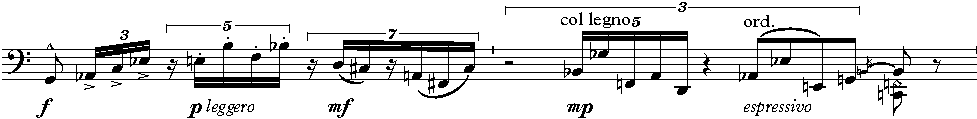
\includegraphics[width=\textwidth]{figures/stingray-example.pdf}
		\caption{Self-derivation in Damiani's \emph{Stingray}.}
	\end{figure}
\end{frame}
